
%%%%%%%%%%%%%%%%%%%% file icsc2017_template.tex %%%%%%%%%%%%%%%%%%%%%
%
% This is the LaTeX source for the instructions to authors using
% the LaTeX document class 'llncs.cls' for contributions to
% the Lecture Notes in Computer Sciences series.
% http://www.springer.com/lncs       Springer Heidelberg 2006/05/04
%
% It may be used as a template for your own input - copy it
% to a new file with a new name and use it as the basis
% for your article.
%
% NB: the document class 'llncs' has its own and detailed documentation, see
% ftp://ftp.springer.de/data/pubftp/pub/tex/latex/llncs/latex2e/llncsdoc.pdf
%
%%%%%%%%%%%%%%%%%%%%%%%%%%%%%%%%%%%%%%%%%%%%%%%%%%%%%%%%%%%%%%%%%%%


\documentclass[runningheads,a4paper]{llncs}

\usepackage{amssymb}
\setcounter{tocdepth}{3}
\usepackage{graphicx}
% \usepackage{url}
\usepackage{hyperref}
\hypersetup{hidelinks}
\usepackage{listings}
%\usepackage{float}
%\restylefloat{figure, lstlisting} 


\newcommand{\keywords}[1]{\par\addvspace\baselineskip
\noindent\keywordname\enspace\ignorespaces#1}

\pagestyle{headings}
% !TeX spellcheck = en_US 

\addtolength{\textfloatsep}{-15px}
\addtolength{\intextsep}{-5px}

\begin{document}

\mainmatter  % start of an individual contribution

% first the title is needed
\title{Frequency Modulation with Feedback in Granular Synthesis}

% a short form should be given in case it is too long for the running head
\titlerunning{FM with Feedback in GS}


% TO GARANTEE THE DOUBLE BLIND REVIEW PROCESS, PLEASE
% KEEP THESE GENERIC AUTHOR NAMES AND INSTITUTIONS

\author{Øyvind Brandtsegg, Victor Lazzarini}
%

\institute{Norwegian University of Science and Technology, Maynooth University \\ \email{oyvind.brandtsegg@ntnu.no, victor.lazzarini@mu.ie}}



\maketitle

\begin{abstract}

The paper investigates audio synthesis with frequency modulation feedback in granular synthesis, comparing it with regular FM feedback. 

\keywords{...}
\end{abstract}


\section{Introduction}
FM synthesis is well known ...(Chowning etc), FM feedback has been explored by \cite{Lazzarini-2024}, frequency modulation in granular synthesis has been briefly explored by \cite{Ervik-Brandtsegg} but it is still a relatively lightly explored topic...here we will look at FM with feedback within granular synthesis as it allows some new means of pitch stabilisation, poses some new problems, and enables some exciting new sonic extensions to both FM and granular synthesis domains.

\section{Basis for comparison}
FM feedback with oscillators and FM feedback in granular synthesis are closely related. Both techniques use a wavetable-reading oscillator to create the output waveform, and the frequency of reading the waveform in the table is modulated by the output waveform via feedback. Granular synthesis differ from the simpler oscillator case in that the wavetable-reading process is reinitialized on every grain, and that an envelope is applied to each grain. The envelope applied to grains can be seen as a form of amplitude modulation, with the envelope shape being used as the modulator waveform. As we shall see, the grain duration has a significant effect on the feedback modulation. The reinitialization of wavetable reading on each grain also means we can have a periodic phase reset. Phase considerations can have a significant effect on feedback modulation, as we will also see later when we apply a phase delay in the modulation feedback loop.

\subsection{\emph{Basics} for comparison}
To enable a comparison between the two techniques, we have attempted to create parameter settings for the granular synthesizer that as close as possible resemble the output from a simple oscillator. In that situation, we can compare differences in parameter settings that apply to both synthesis models. Then, from that comparable situation, we can start to apply parameter changes to the granular process that are not available in the simple oscillator model. By doing this, we can explore in specifics how the granular model extends the notion of FM feedback in the granular domain.

In granular synthesis, the perceived pitch is constituted by the grain rate (\cite{Roads-2001}, \cite{Brandtsegg-particle}). We have thus chosen to let the grain rate be equal to the fundamental frequency of the simple oscillator. Similarly, it makes sense in this context to set the grain frequency (reading speed of the waveform inside each grain) equal to this fundamental frequency. With a the proper envelope, this should allow the granular generator to generate an identical signal as the simple oscillator. The envelope needs to have a smooth fade in and out, and there need to be sufficient overlap between grains to create a constant amplitude in the output. These constraints can be fulfilled in several different ways. With the constraint that the grain rate should equal to the fundamental frequency, the options for the envelope are more limited. We have chosen to use a grain duration of 1.5/grainrate, which means that we have a grain overlap of 33\% (1/3 of the grain will overlap with the next grain). We then use 1/3 of the grain duration for fade in, and equally 1/3 of the duration for fade out. In between fade in and fade out, each grain has a full power sustain period of 1/3 of the grain duration. With an equal power crossfade, we should then be able to recreate a (non granular) waveform. A sigmoid shape is used for the fade in and out of the envelope, to enable equal power crossfading between grains. 

FM feedback with simple oscillators will in its simplest form induce pitch drift, as the output waveform modulate the frequency of the oscillator. This pitch drift can be partly counteracted by recent developments in FM theory (\cite{Lazzarini-2024}), but as this involves an extra step of processing, we don't use it for the simplest possible comparison setup. We will use it as parametric variation when we explore beyond the simplest possible comparison. The pitch drift can also partly be neutralized by adjusting the phase of the feedback modulator. In feedback modulation, adjusting the phase can be done by introducing a small delay in the feedback signal chain. In audio processing the smallest possible feedback delay is 1 sample, so there is inevitably a delay in the feedback in any case. Also, the adjustment of phase of oscillators can be seen as already existing in the simple FM oscillator configuration. Even if it will include an extra processing step (the delay), we consider it to be not more complex than an oscillator with phase control. The delay time is adjusted with respect to the fundamental frequency, so we could call is a phase synced delay. For this reason, delay times are given in fractions of a cycle of the fundamental frequency. 

\subsection{Examples, comparing FM feedback in the two synthesis models}
In our first example we will try to set the parameters so that we get a similar, or comparable, sound from both synthesis models. The example uses an increasing modulation index over time. As can be seen in figure \ref{fig:ex1}, the sidebands show a similar evolution over time. The first sidebands (over the first 1.5 seconds) appear ever so slightly earlier in the oscillator model, but the break to subharmonics (octaviaton) occurs earlier in the granular model (at 1.7 seconds, similarly at 2.7 seconds in the oscillator model). The transition to chaotic behavior occurs almost simultaneously in both models (around 3.5 seconds). The synthesis models use a set of default parameters listed in \ref{lst:defaultparameters} at the very end of the paper, parameter settings deviating from the default setting are listed directly in the figure as nondefault parameters (in between the plots for the granular and oscillator models). The plots show a spectrogram and also zoomed-in snapshots of the waveform at selected locations. The waveform display shows 4 cycles of the waveform in each snapshot, with snapshots being taken every 0.5 seconds of the sound.

\begin{figure}
	\centering
	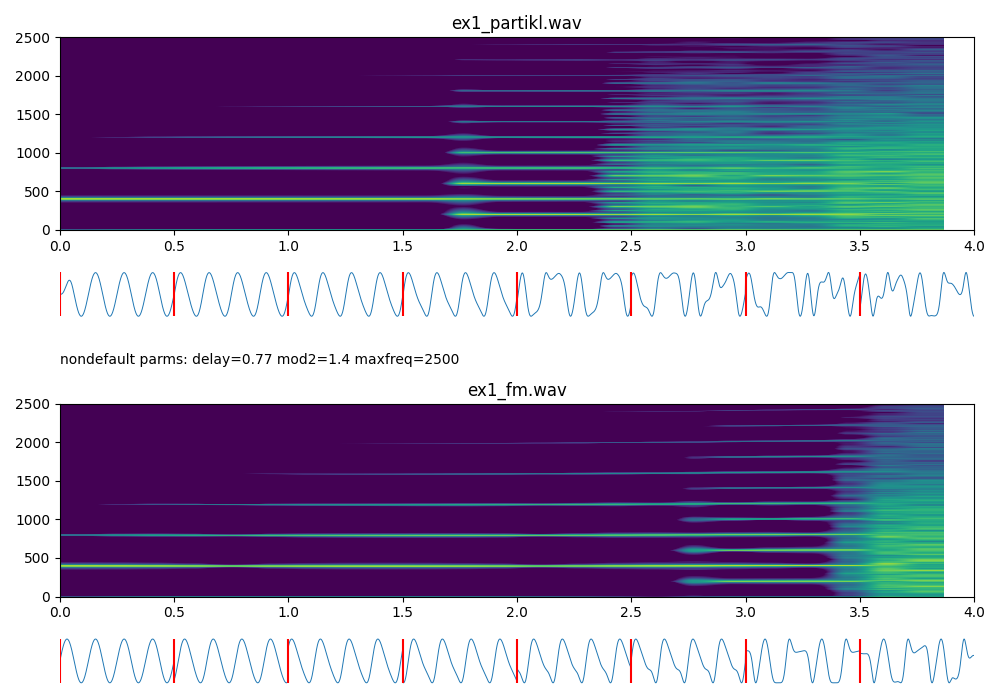
\includegraphics[width=.95\textwidth]{ex1_compare.png}
	\caption{Creating a similar FM feedback sound with the oscillator model and granular model}
	\label{fig:ex1}
\end{figure}

In our second example, we will look at the effect of phase delay and how the granular model has a better ability to create a stable pitch regardless of FM feedback modulation artifacts. The oscillator model pitch drift sets in relatively early (before 1 second) in the example sound, while the granular model keeps a steady pitch throughout. The pitch stability of the granular model relates to the steady grain rate, as explained above. The waveform shape can be modulated without affecting the strictly periodic placement of grains. As can be seen and heard around 2.6 seconds into the sound, the feedback modulation in the granular model leads the waveform close to being trapped/locked at 0Hz. The periodic grain generation, with an envelope securing there is some movement even if the waveform itself could be locked at 0Hz, allow the granular synthesis model to escape the 0Hz "trap".

\begin{figure}
	\centering
	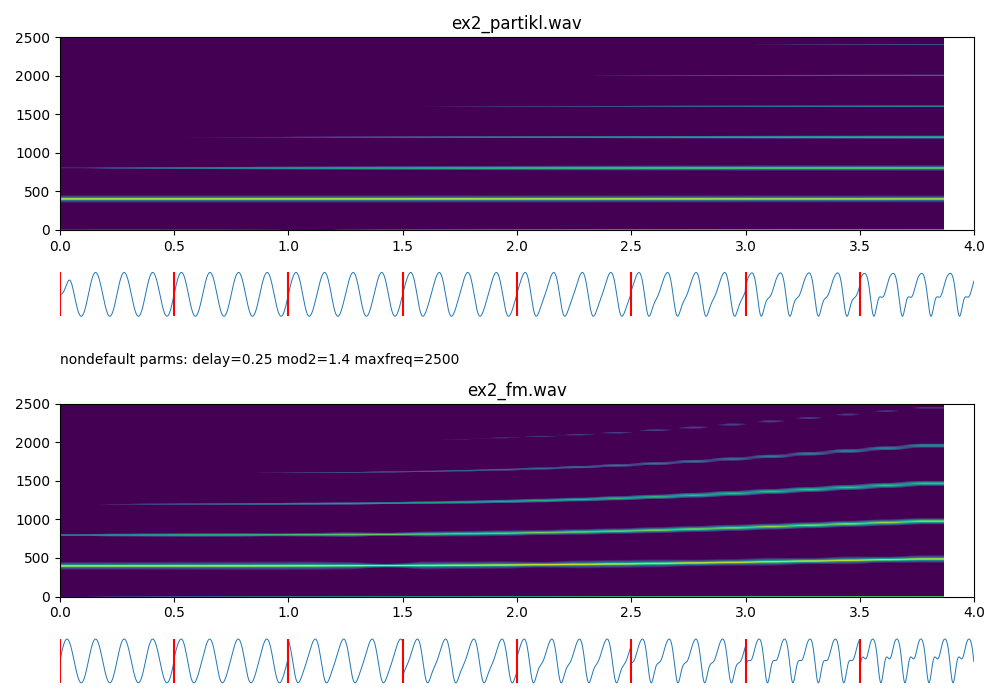
\includegraphics[width=.95\textwidth]{ex2_compare.png}
	\caption{Creating a similar FM feedback sound with the oscillator model and granular model}
	\label{fig:ex2}
\end{figure}

In our third example we  try to see if adding amplitude modulation to the feedback path can stabilize the behavior, as can be learned from \cite{Lazzarini-2024}. Here we go back to the phase delay value used in example 1. As seen in figure \ref{fig:ex3}, the oscillator model keeps a steady pitch (up until mod index $> 1.0$) and also an even and stable spacing of modulation sidebands throughout the example. The granular model displays a splitting of sidebands into subharmonics at half the fundamental frequency (at 1.5 seconds). Interestingly, these sub-bands disappear again, and a steady pitch state is regained until the modulations sidebands split into multiple components towards the very end of the sound.
From this we can assume that the AM in the feedback signal has a different effect in granular than what it has in the oscillator model. The effect of AM in the oscillator model is a more controlled situation, with pitch stability and a constant distance to modulations sidebands. In the granular model, the amplitude modulation has a lesser stabilizing effect. This might relate to the fact that the granular model already has a form of amplitude modulation inherent in the envelope for each grain.

We do note that the oscillator model is not pitch stable at modulation index $> 1.0$. This is to be expected (Victor: can you explain why?). The granular model is pitch stable, even if the harmonic pattern makes the fundamental pitch less prominent at high modulation index. This could indicate that FM feedback in granular synthesis can be utilized to explore new areas of pitch stable FM feedback with high modulation indices.

\begin{figure}
	\centering
	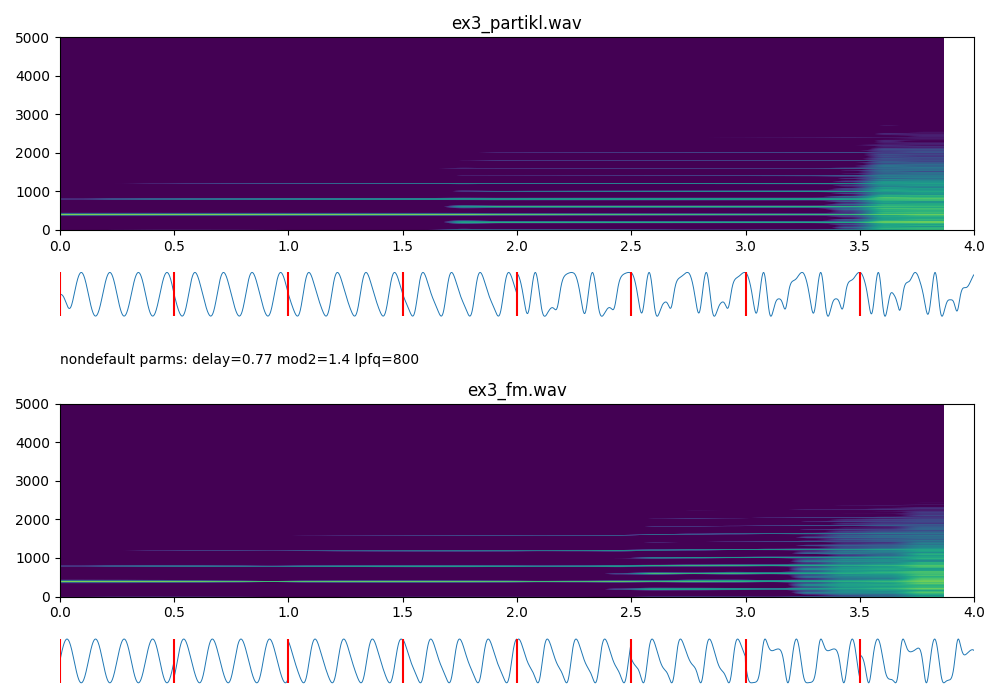
\includegraphics[width=.95\textwidth]{ex3_compare.png}
	\caption{Adding amplitude modulation to the feedback path}
	\label{fig:ex3}
\end{figure}

Adding a lowpass filter to the feedback path can help moderate the chaotic behavior at high modulation indices. As we see in figure \ref{fig:ex4}, it also lower the amplitude of the higher partials generated. An interesting observation is that the sidebands at half the fundamental frequency appears \emph{earlier} with the oscillator model, as compared with the nonfiltered example (figure \ref{fig:ex1}), and we also see a sudden pitch shift occuring at the same time. In the granular model, those sidebands occur at roughly the same time (same modulation index) in the unfiltered and the lowpass example provided here. Pitch is stable throughout the granular example.

\begin{figure}
	\centering
	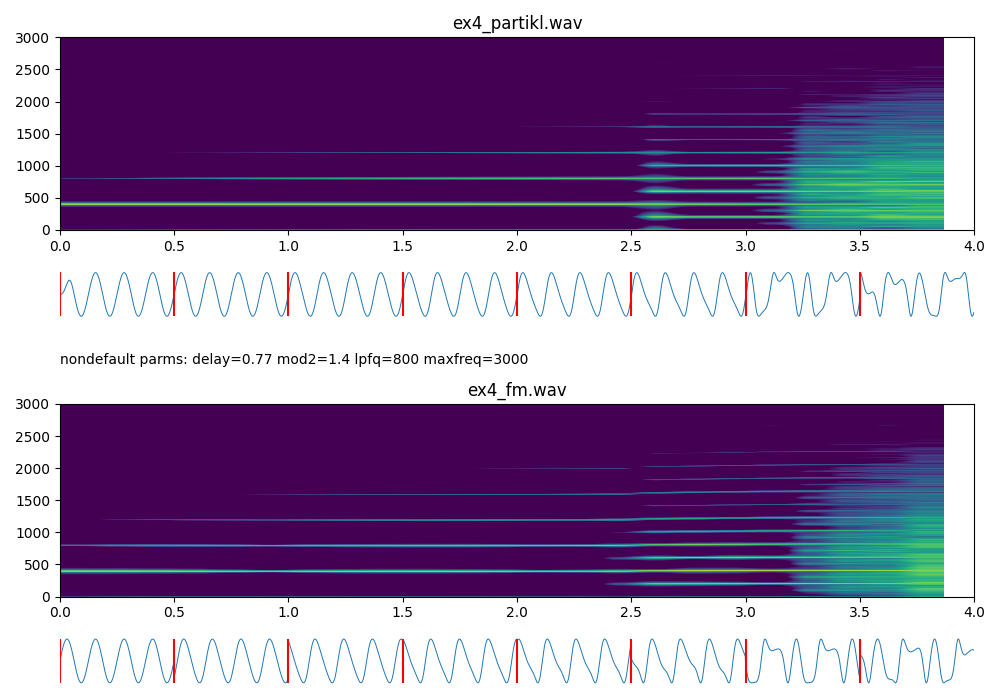
\includegraphics[width=.95\textwidth]{ex4_compare.png}
	\caption{Lowpass filtering the feedback path}
	\label{fig:ex4}
\end{figure}

Another method to moderate chaotic behavior with FM feedback is to add a highpass filter in the feedback path. This will alleviate the effect of DC components resulting from the frequency modulation siddeband at 0Hz.  As can be seen in figure \ref{fig:ex5},  it allows higher modulation index before chaotic behavior in the granular model. Interestingly, the filter seems to disturb the oscillator model, creating sidebands at further subdivisions (1/4?) of the fundamental frequency, and a slightly chaotic behavior already at 2.9 seconds into the sound. Also interesting is that the denser sidebands at 3.0 seconds seems to subside again when modulation index increase further. We have observed this tendency for the complexity of timbre to oscillate slightly with monotonically increasing modulation index. This phenomenon has been observed both with the granular and the oscillator model. It should be mentioned that a filter in the feedback path also will induce delay. We have attempted to compensate for this filter delay in the implementation used for the examples in this paper. The filter delay is frequency dependent, but the delay compensation used here is effective for all frequencies. The required delay time has been calculated from the phase delay at the fundamental frequency of the synthesis example. One should note that some of the artifacts observed might stem from slight variations in phase delay at frequencies corresponding to sideband frequencies.

\begin{figure}
	\centering
	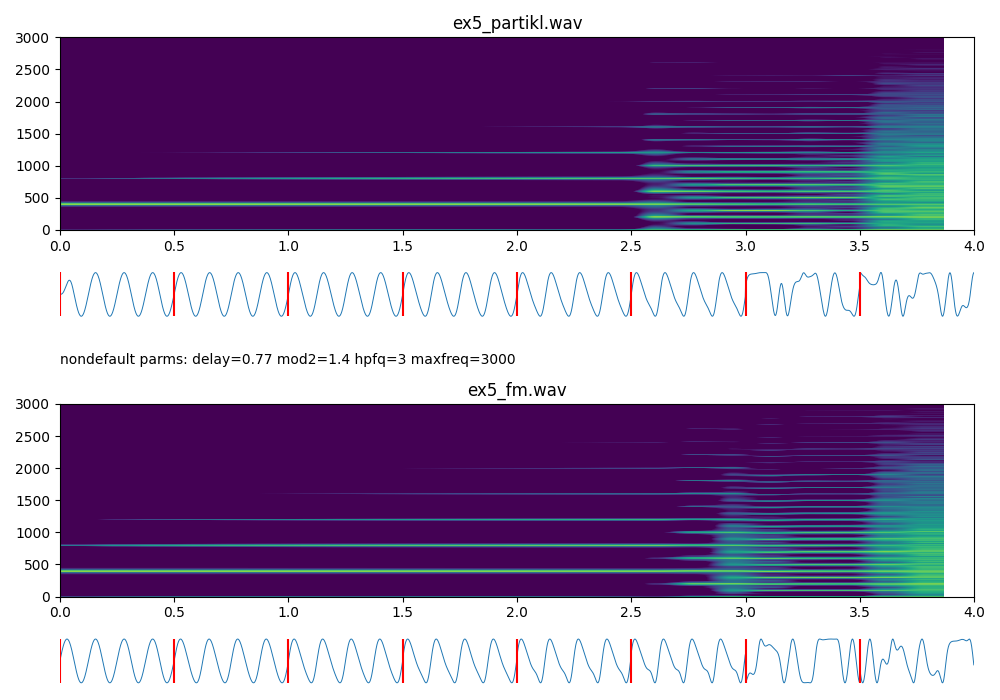
\includegraphics[width=.95\textwidth]{ex5_compare.png}
	\caption{High pass filtering the feedback path.}
	\label{fig:ex5}
\end{figure}

\subsection{Pitfall}
Victor: \\
'*' Do note that phase delay effects have a significant effect on all the previous examples. How to tackle this? Should it be explained in the previous section, or make a separate section on it? \\
'*' What is the theoretical effect of phase delay on regular FM feedback? \\
'*' Also note that some of the effects described are very specific to the parameter settings used. The result may be quite different with slight variation of parameter values. Also note that using a different start value for modulation index will change the behavior: It seems (not surprisingly) like the feedback behavior depends on previous values, that is, the current waveform (at any time) is a result of previous feedback, and as such, a different evolution (over time) of e.g. modulation index will lead to different sonic result (at the same modulation index value). To rephrase: the sonic result of any modulation index value depends on previous values of the modulation index. This leads to a pretty rich variety of potential outcomes, and I'm unsure of how to relate this in a stringent manner when trying to describe specific effects of specific parameter settings.

\subsection{Examples exploring FM feedback extensions in the granular domain}
Exploit the pitch stable behavior to explore situations with higher modulation indices, where pitch instability in the oscillator model makes it impractical.

Grain duration: lowers the effective modulation. But does it allow stable pitch at even higher modulation?

Grain pitch

Phase invert every 2nd grain



\section{Running the provided code examples}
The code examples for this paper can be found in a github repository at \url{https://github.com/Oeyvind/partikkel_fm}. There are Csound orchestra files for FM with granular synthesis and with regular oscillators. To compare the two techniques, it is useful to run both with the same set of parameters (adding only a few extra parameters for granular synthesis), and then compare the generated sound files. The repo contains python files to write score files and render sound with both techniques. This will also display spectrograms for the two generated sound files. The Python files contain default parameter settings as a starting point, and allow parameter modification via command line arguments. For example:
\begin{lstlisting}
python generate_and_compare.py filename cps=200 gr.rate=200
\end{lstlisting}
will modify the fundamental frequency (cps) by setting it to 200Hz, then render sound with both synthesis techniques and display spectrograms for both generated sound files. 

\section{Conclusion}

Lowpass can help\\
Hipass does help in both models\\
AM does help in both models, but only up to mod index = 1 \\

Phase delay ??? complex behaviour. Both models show locking (modulated into stop at zero Hz) behavior when phase delay is less than approx 0.2, but the granular model will keep a steady pitch even if the waveform is almost locked at 0Hz, and thus can regain normal steady pitch operation as the mod index increase even more.

...


\noindent\begin{minipage}{\linewidth}
\begin{lstlisting}[caption=Default parameters for the synthesis models, label=lst:defaultparameters]
"dur" = 4 # duration of the generated sound
"amp" = -6 # overall amplitude
"cps" = 400 # fundamental frequency 
"mod1" = 0 # modulation index at start of sound
"mod2" = 1.5 # modulation index at end of sound
"delay" = 0 # phase delay for the feedback modulator
"lpfq" = 21000 # lowpass filter frequency in feedback path
"hpfq" = 0 #high pass filter frequency in feedback path
"am" = 0 # enable amplitude modulation in feedback path
"gr.pitch" = 400 # grain frequency 
"gr.dur" = 1.5 # grain duration relative to grain rate
"adratio" = 0.5 # attack to decay ratio of grain envelope
"sustain" = 0.33 # sustain length for the grain envelope
"index_map" = 0 # mod index scaling relative to grain dur
"inv_phase2" = 0 # invert the phase of every second grain
	\end{lstlisting}
		\emph{Comments to the default parameters: "cps" sets the fundamental frequency of the oscillator model, and similarly sets the grain rate for the granular model. The filters in the feedback path are completely bypassed when the cutoff frequency is near the extreme setting. This switch has been set to 20kHz for the lowpass filter, and 0.1Hz for the hipass filter. The parameters "gr.pitch", "gr.dur", "adratio", "sustain", "index\_map" and "inv\_phase2" are only used for the granular model. The "index\_map" parameter implements an empirical compensation of the effect grain duration can have on the effective modulation index. Longer grains (overlapping) will lead to a higher amplitude for the feedback signal. The "inv\_phase2" parameter attempts to implement a granular equivalent of the effect that bipolar amplitude modulation can have on the feedback signal, by inverting the phase of every second grain. For this to work correctly, it also doubles the grain rate (thus also halving the grain duration), so it takes two successive grains to synthesize one duty cycle of the waveform.}
	
\end{minipage}


%\pagebreak
\begin{thebibliography}{4}



\bibitem{Lazzarini-2024} Lazzarini, V. and Timoney, J. (2024) \emph{Theory and Practice of Higher-Order Frequency Modulation
	Synthesis}

\bibitem{Ervik-Brandtsegg} Ervik, K. and Brandtsegg, Ø. (2013) \emph{Combining granular synthesis with frequency modulation}. Proceedings of the 2013 Linux Audio Conference. \url{http://lac.linuxaudio.org/2013/papers/42.pdf}

\bibitem{Roads-2001} Roads, C. (2001) \emph{Mocrosound}. MIT Press.  ISBN 0-262-18215-7

\bibitem{Brandtsegg-particle} Brandtsegg, Ø. and Saue, S. and Johansen, T. (2011) \emph{Particle synthesis–a unified model for granular synthesis}. Proceedings of the 2011 Linux Audio Conference. \url{http://lac.linuxaudio.org/2011/papers/39.pdf}

\bibitem{Cabbage-url} Walsh, R. \emph{Cabbage - A framework for audio software development.} \url{https://cabbageaudio.com}

\bibitem{Lazzarini-2016} Lazzarini, V. et al. (2016). \emph{Csound: A Sound and Music Computing System.} Springer.



\end{thebibliography}



\end{document}
